\documentclass{article}
\usepackage[francais]{babel}
\usepackage[utf8]{inputenc}  
\usepackage{listings}
\usepackage{graphicx}
\usepackage{color}
\usepackage{float}
\usepackage{algorithm}
\usepackage[noend]{algpseudocode}

% Style for c code
\definecolor{mygreen}{rgb}{0,0.6,0}
\definecolor{gray}{rgb}{0.5,0.5,0.5}
\definecolor{mymauve}{rgb}{0.58,0,0.82}
\definecolor{backcolour}{rgb}{0.95,0.95,0.92}

\lstdefinestyle{cstyle}{ 
  language=C,
  backgroundcolor=\color{backcolour},   
  basicstyle=\footnotesize,        % the size of the fonts that are used for the code
  captionpos=b,                    % sets the caption-position to bottom
  commentstyle=\color{mygreen},    % comment style
  deletekeywords={...},            % if you want to delete keywords from the given language
  escapeinside={\%*}{*)},          % if you want to add LaTeX within your code
  keepspaces=true,                
  keywordstyle=\color{blue},       % keyword style
  otherkeywords={*,...},           % if you want to add more keywords to the set
  numbers=left,                   
  numbersep=5pt,                   % how far the line-numbers are from the code
  numberstyle=\tiny\color{gray}, % the style that is used for the line-numbers
  rulecolor=\color{black},        
  showspaces=false,               
  showstringspaces=false,          % underline spaces within strings only
  showtabs=false,                  % show tabs within strings adding particular underscores
  stepnumber=1,                    % the step between two line-numbers. If it's 1, each line will be numbered
  stringstyle=\color{mymauve},     % string literal style
  tabsize=2,	                   % sets default tabsize to 2 spaces
  title=\lstname                   % show the filename of files included with \lstinputlisting; also try caption instead of title
}

\lstset{style=cstyle}

\title{Factorisation LU et descente-remontée}
\author{Benjamin \bsc{Angelaud} - Adrien \bsc{Guilbaud}}
\begin{document}
\maketitle

\section{Version Séquentielle}
\subsection{Implémentation de dgetf2\_nopiv}
\paragraph{}La première partie de ce TDP consistait à implémenter une factorisation séquentielle. La première fonction à réaliser a donc été dgetf2\_nopiv(), permettant d'obtenir une factorisation L.U à partir d'une matrice A.  Pour cela, nous réalisons un appel à 2 autres fonctions qui sont dscal() et dger(), que nous avons aussi implémentées (fig \ref{diag:dgetf2}).

\begin{figure}[ht]
  \centering
  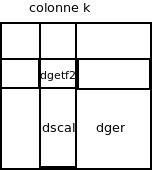
\includegraphics[scale=0.5]{pictures/Diagramme_dgetf2.jpeg}
  \caption{\label{diag:dgetf2} Fonctions utilisées dans dgetf2}
\end{figure}

\paragraph{}Dans la fonction dger() nous avons fait le choix de parcourir sur la boucle intérieur les lignes et les colonnes sur la boucle extérieur pour améliorer nos performances. En effet, comme nous sommes dans le cas où les matrices sont stockées en "column major", il est préférable de stocker une colonne dans le cache et la réutiliser pour le calcul de chaque ligne, plutôt que de devoir recharger toutes les colonnes pour chaque ligne, sachant que les données d'une ligne ne sont pas contiguës en mémoire. Nous le voyons très bien sur la Figure 1 ci-dessous, à partir d'une certaine taille de matrice (ici environ 125) le parcours colonne-ligne devient plus performant. Ceci est du au fait que les colonnes sont réutilisées plusieurs fois pour des calculs alors qu'elle sont stockées dans le cache. C'est aussi pour cela qu'on voit une amélioration très significative de cette méthode, car avant ce seuil le temps passé à stocker les colonnes est plus important que le temps passé à les utiliser pour le calcul.  dgetf2\_nopiv() nous donne donc une factorisation LU séquentielle.

\begin{figure}[!h]
  \begin{center}
    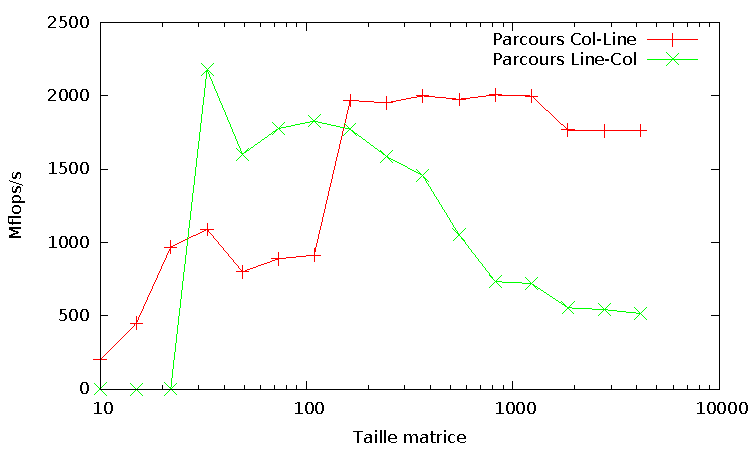
\includegraphics[scale=0.7]{pictures/dger.pdf}
  \end{center}
  \caption{dger: comparaison parcours ligne\_colonne et colonne\_ligne \label{fig:dger}}
\end{figure}

\subsection{Implémentation de dtrsm}En gardant en tête notre objectif final, qui est de résoudre une équation linéaire, la fonction suivante à implémenter était donc dtrsm(), permettant, à partir de la factorisation LU, de résoudre Ax=B. dtrsm() va nous permettre de réaliser le produit d'une matrice triangulaire (supérieure ou inférieure) avec une matrice. Pour se faire, nous avons donc fait le choix d'implémenter la fonction dtrsv() qui permet de réaliser le produit d'une matrice triangulaire (supérieure ou inférieure) avec un vecteur, pour ensuite l'appeler sur chaque vecteur composant notre matrice.

\subsection{Implémentation de dgetrf}Pour pouvoir avoir une factorisation LU par bloc il nous a fallu implémenter une nouvelle fonction réutilisant celles précédemment implémentées (fig \ref{diag:dgetrf}). Ici le but est simple, on fixe une taille de bloc, on effectue un dgetf2\_nopiv() sur les SIZE\_BLOCK première colonnes de la matrice, ensuite on effectue un dtrsm() pour mettre à jour nos SIZE\_BLOCK premières lignes, et pour finir on met à jour le reste de notre matrice avec un dgemm(). Comme nous l'avonc vu précédemment, nous avons implémenté dgetf2\_nopiv() et dtrsm() lors de ce tdp. Pour l'appel à dgemm, nous avons réutilisé notre fonction dgemm\_scalaire mise en place lors du TDP1. Nous sommes conscient que le fait d'utiliser dgemm scalaire nous fait perdre
énormément de performances comparé à une version en blocs, mais lors du TDP1 notre version blocs n'étant pas fonctionnelle nous avons donc réutilisé notre version scalaire.

\begin{figure}[!ht]
  \centering
  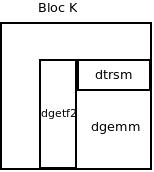
\includegraphics[scale=0.5]{pictures/Diagramme_dgetrf.jpeg}
  \caption{\label{diag:dgetrf} Fonctions appelées dans dgetrf}
\end{figure}

\paragraph{}Nous avons rencontré beaucoup de problèmes sur cette partie de l'implémentation car nos tests de validité n'était pas correct. Néanmoins, nous avons réussi à implémenter une version de dgetrf() totalement fonctionnelle et sur n'importe quelle taille de bloc choisie, nous permettant ainsi de comparer les performances selon la taille des blocs choisie.

\paragraph{}La méthode utilisée pour vérifier la validité de dgetrf() et, en règle plus générale, de toutes nos factorisations LU est la suivante: nous prenons une matrice A contenant des entiers double précision, nous effectuons une copie de cette matrice, puis nous appelons notre fonction pour obtenir notre décomposition LU. Nous faisons ensuite un dgemm sur les matrices triangulaires L et U et comparons le résultat obtenue avec la matrice A initiale.

\paragraph{}L'atout de cette fonction consiste dans le fait d'extraire un dgemm assez "massif" plutôt que d'effectuer un dgetf2\_nopiv() sur toute la matrice. En effet un dgemm se prête parfaitement à une parallélisation alors que dgetf2 contient beaucoup trop de dépendances. C'est en ces termes que nous pourrons extraire de bonnes performances de dgetrf.

\subsection{Implémentation de dgesv}Cette fonction est la fonction "finale" de notre factorisation séquentielle. Elle permet de faire la factorisation LU d'une matrice et de résoudre un système linéaire par descente/remontée. Ici, nous faisons donc appelle à dgetrf() pour obtenir une factorisation LU de notre matrice (préférée à dgetf2\_nopiv() pour des raisons de performances), ensuite nous utilisons dtrsm() deux fois, la première pour obtenir le résultat de y dans Ly=b, puis pour obtenir x dans Ux=y. Une fois ceci terminé nous avons donc résolu notre système linéaire.

\paragraph{}Pour tester la validité de notre dgesv(), nous prenons une matrice A contenant des entiers double précision, un vecteur B avec le même type de données pour obtenir, grâce à notre fonction, le vecteur x résultat. La matrice A et le vecteur B étant modifiés pendant les calculs, nous effectuons une copie initial des deux structures de données. Pour finir nous effectuons un dgemm() sur la matrice A initiale et le vecteur x résultat, et nous comparons le vecteur obtenu avec le vecteur B initial.

\section{Version MPI}
\subsection{Factorisation LU}
Dans un premier temps, nous créons un buffer local dans chaque processus qui contient ses bloc-colonnes locaux selon une distribution en serpentin (fig \ref{diag:serpentin}). Cela permet de rassembler chaque bloc-colonne de façon contigüe en mémoire évitant ainsi les cach-miss provoqués par le parcours la matrice initiale.

\begin{figure}[ht]
  \centering
  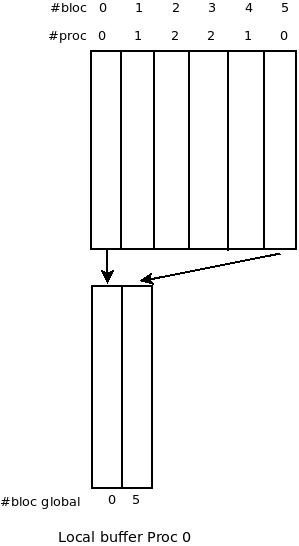
\includegraphics[scale=0.5]{pictures/Diagramme_serpentin.jpeg}
  \caption{\label{diag:serpentin} Exemple de distribution des blocs-colonne pour 3 processus}
\end{figure}


\paragraph{}
Dans l'algo permettant la factorisation LU, (fig \ref{diag:mpi}), nous parcourons tous les bloc-colonnes; quand un bloc appartient à notre processus, nous faisons un dgetrf sur ce bloc puis nous l'envoyons à tous les processus possédant des blocs à droite pour qu'ils mettent à jour leurs blocs. 
Ensuite, nous faisons un dtrsm entre le bloc pivot et tous nos autres blocs situé à droite dans le buffer local puis un dgemm entre la colonne et la ligne du pivot pour mettre à jour la sous matrice. 
\paragraph{}Lorsqu'un processus reçoit un bloc, il effectue un dtrsm entre ce bloc et ses blocs locaux se situant à droite, puis un dgemm entre le bloc reçu et ses blocs locaux.


\begin{figure}[ht]
  \centering
  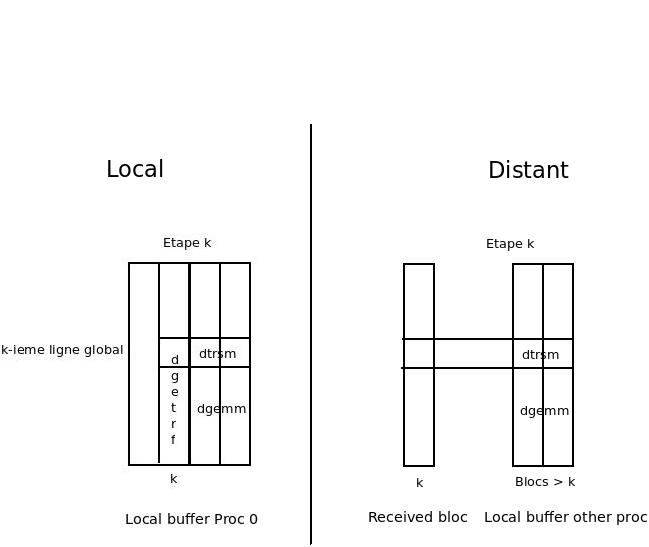
\includegraphics[scale=0.5]{pictures/Diagramme_mpi.jpeg}
  \caption{\label{diag:mpi} Déroulement d'une étape en MPI}
\end{figure}

\subsection{Performances}
Un problème sur Plafrim nous a empêché de réaliser les tests de performances de la partie MPI, nous avons réalisé ces tests sur nos machines personnelles possédant 4 coeurs. Sur la figure \ref{fig:mpi}, nous pouvons observer que lorsque la matrice est assez grande, le temps d'exécution de la factorisation diminue.

\newpage
\begin{figure}[ht]
  \centering
  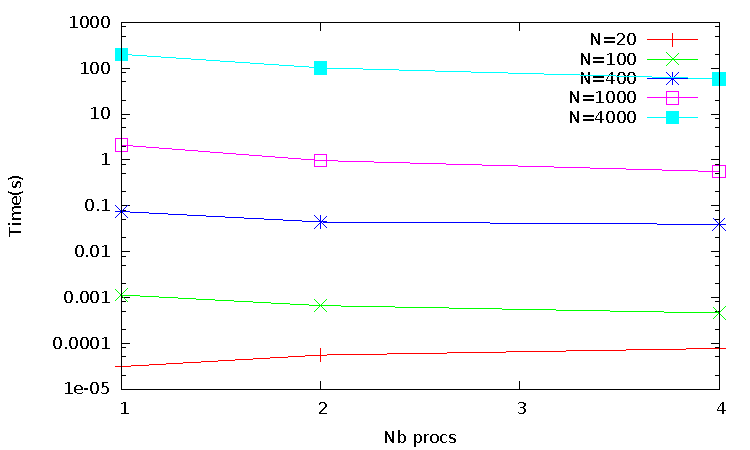
\includegraphics[scale=0.7]{curves/data/mpi.pdf}
  \caption{\label{fig:mpi} Temps d'éxécution en fonction du nombre de processus}
\end{figure}


\section{Améliorations possible}

\paragraph{}La factorisation LU en MPI ne marche que si l'ordre de la matrice est divisible par la taille d'un bloc. Il faudrait donc gérer le cas où il reste un morceau de matrice à attribuer à un processus.
\end{document}